\documentclass[11pt,a4paper]{ivoa}
\input tthdefs

\usepackage{xspace}
% Standard terms used throughout the document,
% defined as macro commands to maintain consistency

% Using non-breaking space character.
% https://stackoverflow.com/a/1012891

\newcommand{\xml} {XML\xspace}
\newcommand{\json} {JSON\xspace}
\newcommand{\yaml} {YAML\xspace}

\newcommand{\datamodel} {data~model\xspace}
\newcommand{\webservice} {webservice\xspace}
\newcommand{\webbrowser} {web browser\xspace}

\newcommand{\uws} {UWS\xspace}
\newcommand{\uwsce} {UWS-CE\xspace}

\newcommand{\ivoa} {IVOA\xspace}
\newcommand{\ivoauws} {IVOA~UWS\xspace}
\newcommand{\ivoavospace} {IVOA~VOSpace\xspace}

\newcommand{\execplanner} {ExecutionPlanner\xspace}
\newcommand{\execworker} {ExecutionWorker\xspace}
\newcommand{\ivoaexecplanner} {IVOA~Execution~Planner\xspace}

\newcommand{\binderhub} {BinderHub\xspace}
\newcommand{\jupyter} {Jupyter\xspace}
\newcommand{\jupyterhub} {JupyterHub\xspace}
\newcommand{\jupyternotebook} {Jupyter~notebook\xspace}

\newcommand{\esap} {ESAP\xspace}
\newcommand{\escape} {ESCAPE\xspace}
\newcommand{\datalake} {DataLake\xspace}
\newcommand{\rucio} {Rucio\xspace}

\newcommand{\python} {Python\xspace}
\newcommand{\pythonprogram} {Python~program\xspace}

\newcommand{\apache} {Apache\xspace}
\newcommand{\spark} {Spark\xspace}
\newcommand{\pyspark} {PySpark\xspace}
\newcommand{\zeppelin} {Zeppelin\xspace}
\newcommand{\zeppelinnote} {Zeppelin~notebook\xspace}

\newcommand{\ocicontainer} {OCI~container}
\newcommand{\docker} {Docker\xspace}
\newcommand{\dockercompose} {Docker~compose\xspace}
\newcommand{\dockercontainer} {Docker~container}

\newcommand{\codeword}[1] {\texttt{#1}}
\newcommand{\footurl}[1] {\footnote{\url{#1}}}

\newcommand{\dataset} {dataset\xspace}
\newcommand{\scienceplatform} {science~platform\xspace}

\newcommand{\executablething}  {\textit{executable~thing}\xspace}

\newcommand{\cpu} {CPU\xspace}
\newcommand{\gpu} {GPU\xspace}

\title{IVOA Execution Planner}

% see ivoatexDoc for what group names to use here; use \ivoagroup[IG] for
% interest groups.
\ivoagroup{GWS}

\author[http://www.ivoa.net/twiki/bin/view/IVOA/DaveMorris]
       {Dave Morris}

\editor[http://www.ivoa.net/twiki/bin/view/IVOA/DaveMorris]
       {Dave Morris}

% \previousversion[????URL????]{????Concise Document Label????}
\previousversion{This is the first public release}

\begin{document}
\begin{abstract}

One of the long term goals of the IVOA has been to enable users to
\textit{`move the code to the data`}.
This is becoming more and more important as the size and complexity
of the \dataset{}s available in the VO increases.
The \ivoaexecplanner provides a step towards making this possible.

The \ivoaexecplanner is designed to address a specific question;
given an \textit{`executable thing`}, e.g. a \pythonprogram or a \jupyternotebook,
what facilities are available to run it?

To do this, the \ivoaexecplanner specification defines
a data model for describing an executable program
and the resources needed to execute it,
and a \webservice API for finding services
that are able to execute it.

Together these components enable a user to ask a simple question
\textit{"Where (and when) can I execute my program?"}

This in turn enables \scienceplatform{}s to share code between them.
Allowing a user to develop their code on one platform and then apply it to a different
\dataset by sending it to execute on another platform.

\end{abstract}

\section*{Acknowledgments}

The authors would like to thank all the participants in the IVOA and ESCAPE projects
who have contributed their ideas, critical reviews, and suggestions to this document.

\section*{Conformance-related definitions}

The words ``MUST'', ``SHALL'', ``SHOULD'', ``MAY'', ``RECOMMENDED'', and
``OPTIONAL'' (in upper or lower case) used in this document are to be
interpreted as described in IETF standard RFC2119 \citep{std:RFC2119}.

The \emph{Virtual Observatory (VO)} is a general term for a collection of
federated resources that can be used to conduct astronomical research,
education, and outreach.
The \href{https://www.ivoa.net}{International Virtual Observatory Alliance (IVOA)}
is a global collaboration of separately funded projects to develop standards and
infrastructure that enable VO applications.

\section{Introduction}
\label{sec:introduction}

The \ivoaexecplanner specification defines two \webservice interfaces, the \execplanner and the \execworker,
and a common \datamodel shared between them for describing executable tasks.

Together these provide a common interface for service discovery, resource allocation and execution scheduling
across a heterogeneous federation of different types of execution platform.

\begin{itemize}
    \item \execplanner \webservice – a discovery service to find execution platforms, allocate resources and schedule execution.
    \item \execworker \webservice – an asynchronous service for executing tasks (based on the \ivoauws pattern).
    \item \execplanner \datamodel – a common data model for describing executable tasks and resource requirements.
\end{itemize}

\subsection{Role within the VO Architecture}
\label{subsec:ivoarole}

% As of ivoatex 1.2, the architecture diagram is generated by ivoatex in
% SVG; copy ivoatex/archdiag-full.xml to role_diagram.xml and throw out
% all lines not relevant to your standard.
% Notes don't generally need this.  If you don't copy role_diagram.xml,
% you must remove role_diagram.pdf from SOURCES in the Makefile.
\begin{figure}
\centering
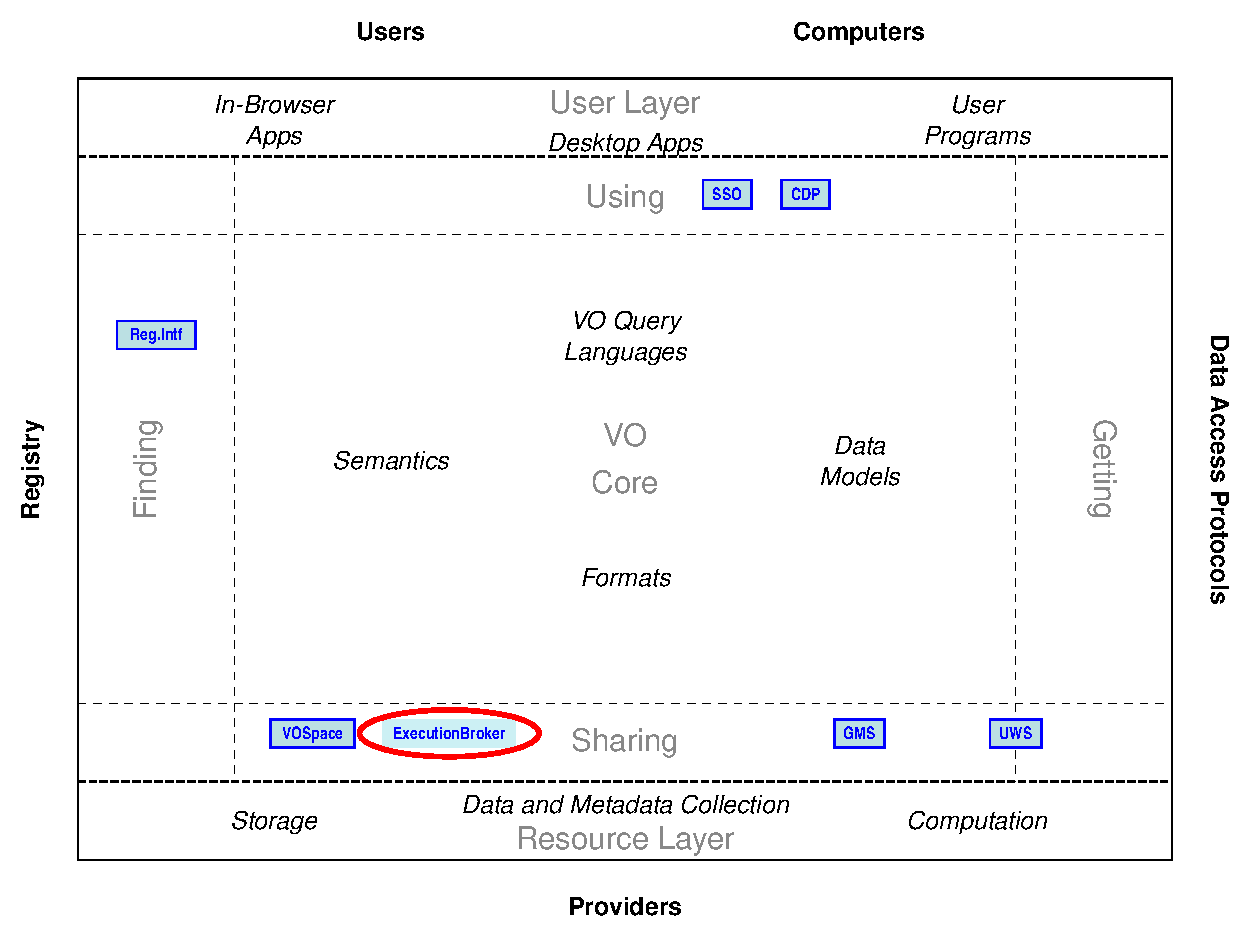
\includegraphics[width=0.9\textwidth]{role_diagram.pdf}
\caption{Architecture diagram showing the \ivoaexecplanner{}'s role in the \ivoa}
\label{fig:archdiag}
\end{figure}

The IVOA Architecture \citep{2010ivoa.rept.1123A} provides a high-level view of how IVOA
standards work together to connect users and applications with providers of data
and services.
Fig.~\ref{fig:archdiag} shows the role the \ivoaexecplanner plays within the this architecture.

In response to the increasing size and complexity of the next generation of science \dataset{}s
many \ivoa participants are developing intergrated \scienceplatform{}s which bring
together the \dataset{}s co-located with the compute resources needed to analyse them.

Many of these \scienceplatform{}s make extensive use of the \ivoa data models,
vocabularies and metadata schema to describe their \dataset{}s,
and use the \ivoa data access services to find and access data from other data providers.
In addition, some of the \scienceplatform{}s make use of the \ivoavospace specification
to manage data transfers to and from local storage co-located with the compute resources.

However, to date the \ivoa does not provide any APIs or \webservice interfaces that
enable \scienceplatform{}s to exchange the software used to analyse the data.
The \ivoaexecplanner provides a step towards making this possible.

This places the \ivoaexecplanner in the same region of the \ivoa architecture
as the \ivoavospace specification \citep{2009ivoa.specQ1007G},
providing an infrastructure level service that enables service discovery,
resource allocation and execution scheduling across a heterogeneous federation
of execution platforms.

The \ivoaexecplanner specification uses the
\ivoa Single-Sign-On standard \citep{2017ivoa.spec.0524T}
for authentication (see section xx )%\ref{subsec:authentication}
and the
\ivoa Credential Delegation Protocol \citep{2010ivoa.spec.0218P}
for delegating authentication credentials to other services.

The \ivoaexecplanner specification also describes how to register
an \execplanner service in the
\ivoa Registry \citep{2009ivoa.spec.1104B}
making it findable within the wider context of the VO.

\subsection{Executable things}
\label{subsec:executablething}

To understand the problem that \ivoaexecplanner is trying to solve
it is useful to describe the concept of an \executablething and what it means in this context.
If we start by thinking of a science domain function that we want to perform.
For example, the mathematical concept of the square root of a number.

We can calculate the square root of a number using a numerical analysis
algorithm that makes successive approximations of the result (cite).

We can write a \pythonprogram to use this algorithm to calculate the square root of a number.
This is the first identifiable \executablething in our example.

To be able to use this \executablething you would need to allocate a computing resource with the appropriate
hardware and software environment. In this case, a computing resource with the \python interpreter installed
along with any 3rd \python modules equired by the program.
This environment is often referred to as the \textit{\python runtime}.

In the context of a \scienceplatform, a common pattern is to provide this environment using an
\ocicontainer\footnote{https://opencontainers.org/},
or
\dockercontainer\footnote{https://docs.docker.com/get-started/what-is-a-container/},
to package the \pythonprogram and the \python runtime together as a single binary object.

This package, or container, is itself an \executablething. One which requires a different execution
environment than the original \python program.
The key concept behind containerization is to package programs together with the software environment
they need as single binary object that interfaces with a standard execution environment,
referred to as the \textit{'container runtime'} or \textit{'container engine'}.

To be able to use this \executablething you would need to allocate a computing resource with the appropriate
hardware and software environment. In this case, a computing resource with the OCI container runtime installed.

We could also create a \jupyternotebook that demonstrates how to use our \pythonprogram.
This is the third \executablething in our example.
One which provides an interactive environment for the user to experiment with.

As before, to be able to use this \executablething we would need to allocate a computing resource with
the appropriate hardware and software environment.
In this case, a computer with the \jupyternotebook platform installed along with all the 3rd \python modules
needed by our \pythonprogram.
In the context of a \scienceplatform, a common pattern is to provide this environment as a \webservice
that allows the user to connect to the \jupyternotebook via a \webbrowser.

From one algorithm that implements a science domain function, we have created three different \executablething{}s.
A \python program, an \ocicontainer packaging the \pythonprogram and its dependencies, and an interactive \jupyternotebook
that demonstrates how to use the \python progran.

Each of these \executablething{}s requires a different computing environment to execute.
A basic \python runtime, the \ocicontainer runtime, and a \jupyternotebook service.

We may also want to consider the data that we are applying the algorithm to.
If we are learning how to use algorithm, then a basic computing resource will be sufficient
to experiment with.
However, if we have a \dataset of ten million numbers that we want to process, then we may
need to consider adding extra storage to handle the input data and the results.
For a large \dataset it may also be worth using a \gpu to accelerate the calculation steps
for such a large \dataset.

The \ivoaexecplanner \datamodel provides a way to describe what each of these \executablething{}s
is and what resources are needed to execute it.

The description for each \executablething can include things like number of \cpu cores and
amount of memory it needs, whether it needs a \gpu, the location of the input data,
the storage space needed to perform the calculation and the storage space needed to save the results.

This metadata description can be passed to the \ivoaexecplanner services to discover if they
are able to provide the resources required to execute this particular \executablething.

For more details on the \ivoaexecplanner \datamodel see section xx.

\appendix
\section{Changes from Previous Versions}

No previous versions yet.
% these would be subsections "Changes from v. WD-..."
% Use itemize environments.


% NOTE: IVOA recommendations must be cited from docrepo rather than ivoabib
% (REC entries there are for legacy documents only)
\bibliography{ivoatex/ivoabib,ivoatex/docrepo}


\end{document}
